\documentclass[a4paper,twoside,11pt]{article}
\usepackage[english]{babel}
\usepackage[utf8]{inputenc}
\usepackage[T1]{fontenc}
\usepackage{lmodern}
\usepackage[noadjust]{cite}
\usepackage{todonotes}
\usepackage{natbib}
\usepackage{url}
\usepackage{amsmath}
\usepackage{graphicx}
\usepackage{textcomp}
\graphicspath{{images/}}
\usepackage{parskip}
\usepackage{fancyhdr}
\usepackage{vmargin}
\usepackage{tikz}
\usepackage{pstricks}
\usepackage{pst-optexp}
%\usepackage{auto-pst-pdf}
%\setmarginsrb{3 cm}{2.5 cm}{3 cm}{2.5 cm}{1 cm}{1.5 cm}{1 cm}{1.5 cm}
\setmarginsrb{2.5 cm}{2.5 cm}{2.5 cm}{2.5 cm}{1 cm}{1 cm}{1 cm}{1 cm}


\usepackage{multicol}
%\usepackage{nonfloat}

%\usepackage{amsfont}
\usepackage{amssymb}

\usepackage[none]{hyphenat}
\usepackage{amsmath}

\usepackage[scientific-notation=true]{siunitx}
\usepackage{subcaption}
%\usepackage[table,xcdraw]{xcolor}
%\usepackage[squaren,Gray]{SIunits}
\usepackage{todonotes}
\usepackage{color}
\usepackage{colortbl}
\usepackage{diagbox}
\usepackage{multirow}
\usepackage{glossaries}
\makeglossaries
\input{glossaire.gls}

\pagestyle{fancy}
\fancyhead{}
\fancyfoot{}
\fancyhead[LE,RO]{\thepage}
\fancyhead[LO,RE]{\rightmark}

\title{Simulation and characterization of integrated optics beam combiners for astrointerferometry}								% Title
\author{Thomas Poletti}								% Author
\date{\today}											% Date

\makeatletter
\let\thetitle\@title
\let\theauthor\@author
\let\thedate\@date
\makeatother


\renewcommand{\headrulewidth}{0pt}
\renewcommand{\footrulewidth}{0pt}

\graphicspath{ {images/} }

\newcommand\frontmatter{%
    \clearpage
  %\@mainmatterfalse
  \pagenumbering{roman}}

\newcommand\mainmatter{%
    \clearpage
 % \@mainmattertrue
  \pagenumbering{arabic}}

\newcommand\backmatter{%
  \if@openright
    \clearpage
  \else
    \clearpage
  \fi
 % \@mainmatterfalse
   }

   
\usepackage[linktoc=all]{hyperref}
\hypersetup{
    colorlinks,
    citecolor=black,
    filecolor=black,
    linkcolor=black,
    urlcolor=black
}

\usepackage[nottoc]{tocbibind}




\makeglossary

\begin{document}

%\listoftodos
%%%%%%%%%%%%%%%%%%%%%%%%%%%%%%%%%%%%%%%%%%%%%%%%%%%%%%%%%%%%%%%%%%%%%%%%%%%%%%%%%%%%%%%%%

\begin{titlepage}

	\begin{minipage}{0.5\textwidth}
		\begin{flushleft} 
    %\vspace*{0.5 cm}
    \includegraphics[scale = 0.6]{phelma.png}\\[1.0 cm]	% University Logo
			\end{flushleft}
			\end{minipage}~
			\begin{minipage}{0.5\textwidth}
            
			\begin{flushright} 
    
    %\vspace*{0.5 cm}
    \includegraphics[scale = .9]{university.png}\\[1.0 cm]	% University Logo
		\end{flushright}
        
	\end{minipage}\\[3 cm]
	
    \centering
    \vspace*{0.5 cm}
	\rule{\linewidth}{0.2 mm} \\[0.4 cm]
	{ \huge \bfseries \thetitle}\\
	\rule{\linewidth}{0.2 mm} \\[1.5 cm]
    \textsc{\Large I. Physikalisches Institut \\
Universität zu Köln}\\[5 cm]	% University Name
	%\textsc{\Large Grenoble INP-Phelma}\\[0.5 cm]				% Course Code

	
	\begin{minipage}{0.4\textwidth}
		\begin{flushleft} \large
			\emph{Author :} \\
			Thomas Poletti\\
  %           13103057\\
          M1 Physics and NanoSciences\\
          School-year 2017-2018\\
   %         Semester\\
			\end{flushleft}
			\end{minipage}~
			\begin{minipage}{0.4\textwidth}
            
			\begin{flushright} \large
   			\emph{Supervisor:}\\
			Pr. Dr. Lucas Labadie\\
            labadie@ph1.uni-koeln.de\\
		\end{flushright}
        
	\end{minipage}\\[2 cm]
	
    
    
	
\end{titlepage}

\frontmatter
\begin{abstract}
   abstract-text
\end{abstract}
\renewcommand{\abstractname}{Résumé}
\begin{abstract}
   Résumé ici
\end{abstract}
\renewcommand{\abstractname}{Introduction}

\newpage
\tableofcontents
\listoffigures
\listoftables

\clearpage

\mainmatter

\begin{abstract}
Since antiquity and down to our time, astronomers always tried to see further and further in space requiring more and more sensitive instruments. Increasing the telescope diameter is one way to reach higher angular resolution but in the same time make it more sensitive to atmospheric turbulence. Therefore even with the recent progress in adaptative optics, today's largest telescopes can only resolve few of the brightest and nearest stars. 

Using individual telescopes to form an interferometer, the resolution is determined by the distance between the telescopes. Until recently the instruments combining the light from individual telescopes were based on costly and cumbersome bulk optics. The recent advances in manufacturing integrated-optics and especially in laser processing have resulted in new instruments that are operational on sky and delivering higher quality results. 

The purpose of this work is to optimise and characterise the performance of \gls{io} beam combiners and especially one promising type of component called \gls{dbc}. Allowing to retrieve the astronomical parameters without scanning fringes these components could allow to observe fast varying objects. Moreover their structure without bending should provide high throughput thus higher quality measurements. 

This report is organised in three parts. In the first part will be presented the motivation and the basis of astronomical interferometry. In the second part simulation results of the \gls{dbc} as well as its optimisation will be discussed. In the last part the experimental characterisation of the \gls{dbc} and its accuracy in retrieving the astronomical parameters will be demonstrated.

\end{abstract}


\section{Fundamentals of astro-interferometry}
All the development of astro-interferometry is essentially based on one fundamental theorem : the Van Cittert-Zernike theorem. This theorem links the spatial coherence of a far source to its angular brightness distribution. In this section will be explained the limitation of one individual telescope in term of resolution and then introduce the advantages of interferometry. This section is based on \cite{Glindemann} and lectures given by J.P. Berger at Grenoble-INP Phelma. In order to fully understand the concepts lets first introduce the Mutual coherence function.

	\subsubsection{Mutual coherence function}
Lets consider the light field by its optical disturbance function $u(\vec{r},t)$ at position $\vec{r}$ and time $t$. The optical disturbance is proportional to the electrical and magnetic field of the light.
Lets suppose a far, coherent source illuminating two thin holes situated at position $\vec{r_1}$ and $\vec{r_2}$ (like the young experiment) and forming fringe pattern on a screen. At a point P ant time t of the screen the intensity of the light can be expressed by :
$I(P) = \left< u(P,t)u^*(P,t) \right>$ which can be rewritten if we consider the holes thin enough that the field is constant on their respective surface :
$$
I(P) = \left< \left| u(\vec{r_1},t-\tau_1) \right|^2 \right> + \left< \left| u(\vec{r_2},t-\tau_2) \right|^2 \right> +2\mathcal{R}\left( \left< \left| u(\vec{r_1},t-\tau_1)u^*(\vec{r_2},t-\tau_2) \right| \right> \right)
$$
where $\tau_1$ and $\tau_2$ refers to the travel time of the wave from the pin hole to the point P. The last term of this equation is a term of coherence representing the spatial and spectra properties of the source. From this equation we can generalise the measurement of the coherence of a source by introducing the mutual coherence function (MCF) :
\begin{equation}
\Gamma(\vec{r_1},\vec{r_2}, \tau) = \left< u(\vec{r_1},t+\tau)u^*(\vec{r_2},t)\right> = \lim\limits_{T\rightarrow +\infty}\int_{-T}^T u(\vec{r_1},t+\tau)u^*(\vec{r_2},t)dt
\end{equation} 

In the case of astrointerferometry the two pinholes refers to the telescopes and the source to the observed object. The distance between both telescopes is called the baseline vector $\vec{B}=\vec{r_1}-\vec{r_2}$. 

	\subsubsection{Van Cittert-Zernike theorem}
Now that the MCF has been defined the most fundamental theorem of modern optic can be introduced. We will consider the Van Cittert-Zernike theorem in an adapted to astronomy form. We will consider a surface emitting light. Under the following assumption :
\begin{itemize}
\item[-]The source is incoherent ($\Gamma(P_1,P_2,\tau) = 0 \quad P_1 \neq P_2$ for all $\tau$)
\item[-]The source is small compared to the distance of observation (Fresnel approximation)
\item[-]The source spectral bandwidth is much smaller than its average frequency (quasi-monochromatic approximation).
\end{itemize}

\begin{figure}[htbp!]
\centering
\includegraphics[scale=.3]{../images/scheme.png}
\caption{Scheme of the principle of stellar interferometry. (adaptated from \url{https://fr.wikipedia.org/wiki/Interférométre_optique_à_longue_base})}
\end{figure}

Under those assumptions the Van Cittert-Zernike theorem states that :
$$
\mu(\vec{B}) = \frac{\Gamma(\vec{B},0)}{\sqrt(\Gamma{\vec{r_1},\vec{r_1},0)\Gamma(\vec{r_2},\vec{r_2},0)}} = \frac{\int I_b(\vec{\alpha}) e^{-ik\vec{B} \cdot \vec{\alpha}}}{d\vec{\alpha}}
$$

where alpha is the angle between the line of sight and a point on the observed source and $\mu$ the normalised MCF at $\tau=0$, called the visibility function. $I_b(\vec{\alpha})$ is the angular brightness distribution of the source. This is the force of this theorem, linking the angular brightness distribution of an object to the shape of its interferometric signal. The source can be seen as an infinity of points each interfering at the telescope recombination point. But due to their different position their interferogram are shifted relatively to each other reducing the global visibility. This is this effect that the Van Cittert-Zernike theorem means. Thus the amplitude of visibility $\left| \mu \right|$ lay between 0 and 1.

This theorem explain the usability of interferometry to astronomical purpose but it doesn't explain it's main advantage : an increased angular resolution. 

\begin{figure}[htbp!]
\centering
\includegraphics[scale=.3]{../picture/airy.pdf}
\caption{Left : Airy disk / PSF of a circular aperture. Center : Case of the Rayleigh criterion (resolved source). Right : case of an unresolved source}
\label{fig:airy}
\end{figure}

	\subsubsection{Spatial resolution}
Lets now take a simplified example of an individual telescope whose pupil is a disk of diameter D. Fourier's optics tells us that the point spread function (PSF) of such an aperture is a function called Airy's function (see Fig\ref{fig:airy}). 

In the case of 2 source observed, one can define the resolution of the telescope as its capacity to separate two punctual sources. This criterion is called the Rayleigh criterion and is defined as the angular separation such as the first "0" of the image of the first source is at the position than the maximum of the image of the second source. This correspond to an angular resolution of $\Delta \alpha = \frac{1.22\lambda}{D}$. 

One can also define the telescope by its optical transfer function. Doing so it is easy to show that the circular aperture act as a low pass filter (spatial frequency) with a cut off frequency of $f_c = \frac{D}{\lambda}$

When it comes to interferometry with two telescopes separated by a distance $\vec{B}$ (speaking of the effective baseline) observing two stars of same flux separated by a distance $\vec{\rho}$, the visibility function is $\mu(\vec{f})=cos(\vec{f}\dot\vec{\rho})$ where $\vec{f}$ if the spatial frequency vector $\vec{f} = \frac{\vec{B}}{\lambda}$ ($\vec{B}$ and $\vec{\rho}$ are vectors defined in the observation plan). In the particular case where $\vec{\rho}= \frac{\lambda}{2\left|\vec{B}\right|} \frac{\vec{B}}{\left|\vec{B}\right|}$ the visibility is equal to zero. Therefore we can deduce that the interferometer formed by two telescopes separated by a distance B is equivalent to an individual telescope of diameter B.  

An interferometer formed by two telescopes separated by a distance B has a resolution of $\frac{lambda}{2B}$ and give access to spatial frequency per $\frac{B}{\lambda}$ per radians of the source. To be able to fit models to measured visibility and to reconstruct an image of the observed object one must do measurements for as many baselines as possible (and also as as many wavelength as possible). The purpose of the work presented in this report is to develop a component able to combine at least 4 telescopes (6 different baselines) at the same time making it able to observe fast varying object.




\section{Simulation of the DBC}
    
    The discrete beam combiner is a component made of multiple straight single-mode waveguides close to each other. It has been demonstrated that in the case of a $N$ telescope \gls{dbc}, an array of more than $N^2$ waveguides is needed for efficient operation of the \gls{dbc} \cite{minardi1}. But at this point it hasn't been studied the impact of other geometrical parameters such as the spacing between each waveguides. 
    
    The component studied is formed of 23 outputs and four inputs to combine the light from four individual telescopes. A cross-section of it is shown on Fig. \ref{tikz:ZigZagCrossSection}. Both the input configuration and the "Zig-Zag" shape have already been optimised. After a brief explanation of the theory behind the \gls{dbc} we will focus on optimising it regarding $P_x$, $P_y$, $width$, $height$ and the length of the \gls{dbc} part (the notations refers to Fig. \ref{tikz:ZigZagCrossSection}) in the case of monochromatic light. In a second part the performances of the optimised component regarding the bandwidth of the input light are simulated. All simulation are performed using the commercial software Beamprop\textcompwordmark{} in scalar mode (a full-vectorial mode would have been more accurate but didn't show much different results for both TE and TM polarisation regarding the condition number of the \gls{V2PM} -see next section-), correlation mode and transparent boundary condition. The grid size was chosen as a balance between computation time and accuracy. The waveguides are simulated by a step-index core.
    \begin{figure}
\resizebox{\textwidth}{!}{
  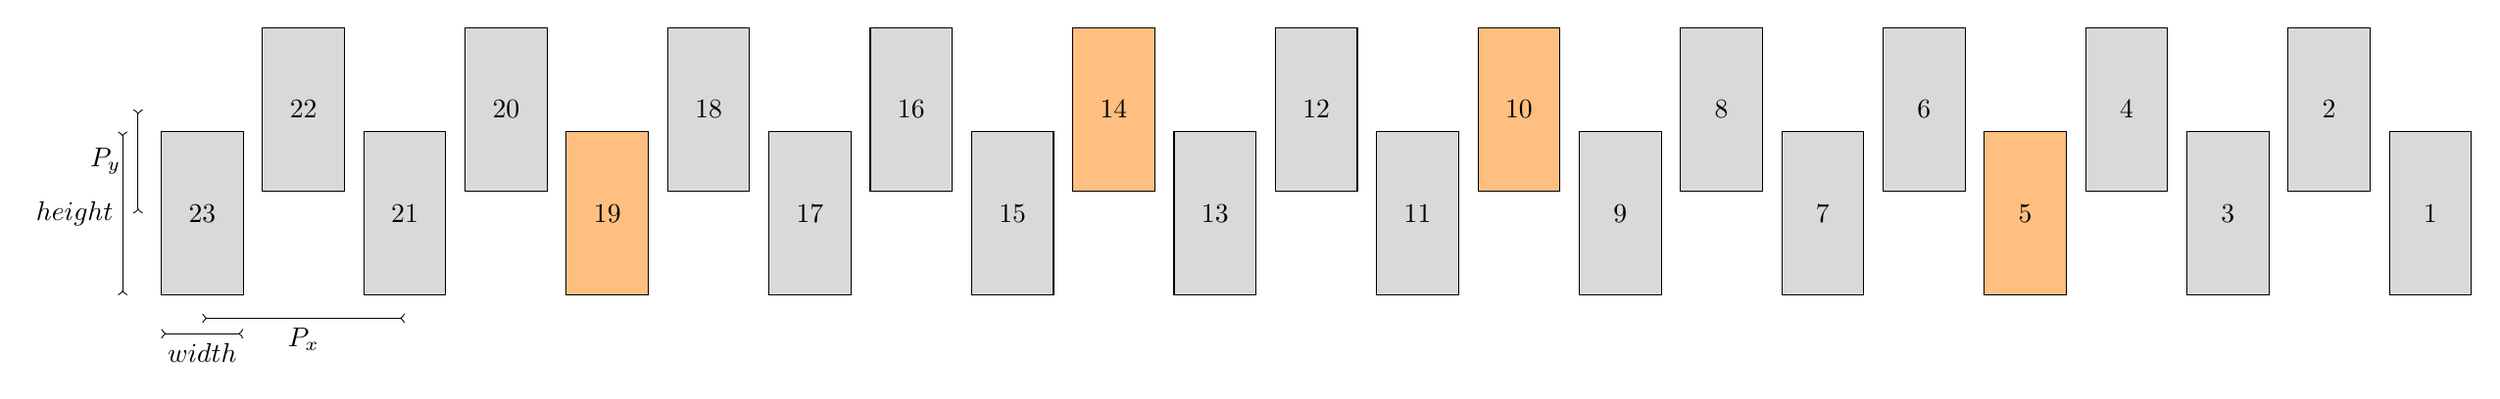
\begin{tikzpicture}

  \def \Px {21/8}
  \def \Py {10.8/8}
  \def \width {8.5/8}
  \def \height {17/8}

  \foreach \i in {0, 1, 2 ,3 ,4 ,5, 6, 7, 8 ,9 ,10, 11}
  {
    \draw[fill=gray!30] (\i * \Px, 0) rectangle (\width + \i * \Px,
    \height);
    \pgfmathtruncatemacro\num{23-2*\i}
    \ifthenelse{\num = 19 \OR \num = 5}{\draw[fill=orange!50] (\i * \Px, 0) rectangle (\width + \i * \Px,
    \height);}{}
    \draw (\width / 2 + \i * \Px, \height / 2) node {\num};
  }

  \foreach \i in {0, 1, 2 ,3 ,4 ,5, 6, 7, 8 ,9 ,10}
  {
   \draw[fill=gray!30] (\Px / 2  + \i * \Px, \Py )
    rectangle (\Px / 2 + \width  + \i * \Px, \Py + \height );
    \pgfmathtruncatemacro\num{22-2*\i}
    \ifthenelse{\num = 14 \OR \num = 10}{\draw[fill=orange!50] (\Px /
      2  + \i * \Px, \Py ) rectangle (\Px / 2 + \width  + \i * \Px, \Py + \height );}{}
    \draw (\width / 2 +\Px / 2 +\i * \Px, \Py + \height / 2) node {\num};
  }

  \draw[>-<] (\width / 2,-.3) -- (\Px + \width / 2,
  -.3);
  \draw (\Px / 2 + \width / 2, -.3) node[below] {$P_x$};
  \draw[>-<] (-.3 , \height / 2) -- (-.3,  \height / 2 + \Py);
  \draw (-.4, \Py /2 + \height / 2) node[left]
  {$P_y$};

  \draw[>-<] (0,-.5 ) -- (\width, -.5);
  \draw (\width / 2, -.5) node[below] {$width$};

  \draw[>-<] (-.5,0) -- (-.5, \height);
  \draw (-.5, \height/2) node[left] {$height$};
\end{tikzpicture}}
\caption{The Zig-Zag array cross section with the numbering
  convention. The four input waveguides  are displayed in orange.}
\label{tikz:ZigZagCrossSection}

\end{figure}


    \subsection{Monochromatic light}

    In this section is shown the impact on the performances of the \gls{dbc} regarding its geometry. Two main parameters are studied, the condition number of the \gls{V2PM} and the throughput as it hadn't been done before. 
        \subsubsection{Mathematical formalism}\label{sec:mathmono}
        As stated before the "Zig-Zag" \gls{dbc} is composed of 23 outputs and can combine the light from 4 individual telescopes. This component has the particularity that all the information about the coherence function of the studied object is included in the way the 23 outputs are related to each other \cite{tatulli}. In the case of monochromatic light the theory is exact. We will do a brief overview of the theoretical background in this part. For further reading the reader can refer to \cite{tatulli, saviauk, Diener2017}.

In this part we will consider the light combined from the input $A$ and $B$ at the $n^{th}$ output. In that case the intensity $I_n$ at the output can be expresed as :
\begin{equation}\label{eq:intermono}
 I_n = \kappa_AI_A+\kappa_BI_B+2\sqrt{\kappa_AI_A\kappa_BI_B}V_{AB}^{inst}V_{AB}^{obj}\cos(\phi_{AB}^{inst}+\phi_{AB}^{obj})
\end{equation}

In this equation $\kappa_i$ is the transmission coefficient from the input $i$ to the considered output. $inst$ and $obj$ relates the visibility/phases of the instrument and of the observed object. Equation \ref{eq:intermono} can easily be reduced to Eq.\ref{eq:intermonoreduced} in which the produce of the instrumental and object visibility are reduced in $V_{AB}$.

\begin{equation}\label{eq:intermonoreduced}
  I_n = \kappa_AI_A+\kappa_BI_B+2\sqrt{\kappa_AI_A\kappa_BI_B}V_{AB}\left(\cos(\phi_{AB}^{inst})\cos(\phi_{AB}^{obj})-\sin(\phi_{AB}^{inst})\sin(\phi_{AB}^{obj})\right)
\end{equation}

From Eq.\ref{eq:intermonoreduced} the problem of getting the object mutual coherence function can be reduced to the produce of a matrix and a vector. 
Thus the
characteristics of the input fields can be linked to the output
intensities by the relation :
\begin{equation}
  \vec{I} = V2PM \times \vec{V}
\end{equation}
In which $\vec{I} = (I_1,...I_M)^T$ represent the intensities at the M outputs, \\ \resizebox{\textwidth}{!}{ $\vec{V} =
(I_1,...,I_M,V_{12}^{obj}\sqrt{I_1I_2}cos(\Phi_{21}^{obj}),V_{12}^{obj}\sqrt{I_1I_2}sin(\Phi_{21}^{obj}),...,V_{N-1,N}^{obj}\sqrt{I_{N-1}I_N}cos(\Phi_{N,(N-1)}^{obj}),V_{N-1,N}^{obj}\sqrt{I_{N-1}I_N}sin(\Phi_{N,(N-1)}^{obj}))$}
and the visibility to pixel matrix V2PM represent the beam combiner's properties. An example of a V2PM for an hypothetical beam combiner
with 3 inputs and 2 outputs is displayed in Figure \ref{v2pm.expl}

\begin{figure}[h]
\begin{equation*}
\resizebox{\textwidth}{!}{
 $ \begin{pmatrix}
  \kappa_{11} & \kappa_{21} & \kappa_{31} &
  2V_{12}^{1}\sqrt{\kappa_{11}\kappa_{21}}cos(\Phi_{12}^{inst}) &
  -2V_{12}^{1}\sqrt{\kappa_{11}\kappa_{21}}sin(\Phi_{12}^{inst}) &
  2V_{13}^{1}\sqrt{\kappa_{11}\kappa_{31}}cos(\Phi_{13}^{inst}) &
 - 2V_{13}^{1}\sqrt{\kappa_{11}\kappa_{31}}sin(\Phi_{13}^{inst}) &
  2V_{23}^{1}\sqrt{\kappa_{21}\kappa_{31}}cos(\Phi_{23}^{inst}) & -2V_{23}^{1}\sqrt{\kappa_{21}\kappa_{31}}sin(\Phi_{23}^{inst})\\
  \kappa_{12} & \kappa_{22} & \kappa_{32} &
  2V_{12}^{2}\sqrt{\kappa_{12}\kappa_{22}}cos(\Phi_{12}^{inst}) &
  -2V_{12}^{2}\sqrt{\kappa_{12}\kappa_{22}}sin(\Phi_{12}^{inst}) &
  2V_{13}^{2}\sqrt{\kappa_{12}\kappa_{32}}cos(\Phi_{13}^{inst}) &
 - 2V_{13}^{2}\sqrt{\kappa_{12}\kappa_{32}}sin(\Phi_{13}^{inst}) &
  2V_{23}^{2}\sqrt{\kappa_{22}\kappa_{32}}cos(\Phi_{23}^{inst}) &   -2V_{23}^{2}\sqrt{\kappa_{22}\kappa_{32}}sin(\Phi_{23}^{inst})

\end{pmatrix}
$}
\end{equation*}
\caption{An hypothetical V2PM matrix for a 3 to 2 beam combiner. All visibility and phases in the matrix are the instrumental ones.}
\label{v2pm.expl}
\end{figure}

One can find the \gls{P2VM} by inverting the V2PM
matrix with the relation \ref{eq:p2vm} and then the astronomical
information from $\vec{V}$. To be consistent with the notation introduced in \cite{saviauk},   $\vec{V} =
(\Gamma_{11},...,\Gamma_{MM},\mathcal{R}\Gamma_{12},\mathcal{I}\Gamma_{12},...,\mathcal{R}\Gamma_{N(N-1)},\mathcal{I}\Gamma_{N(N-1)})$ the object phase and visibility can be extracted by :
$$
V_{ij}^{obj} = \sqrt{\frac{(\mathcal{R}\Gamma_{ij})^2+(\mathcal{I}\Gamma_{ij})^2}{\Gamma_{ii}\Gamma_{jj}}} \qquad
\Phi_{ij}^{obj} = arctan(\frac{\mathcal{I}\Gamma_{ij}}{\mathcal{R}\Gamma_{ij}}) \quad i\neq j
$$

\begin{equation}
  P2VM = (V2PM^T\times V2PM)^{-1}\times V2PM^{T} \label{eq:p2vm}
\end{equation}  

In the light of this formalism the retrieved coherence function from the \gls{P2VM} can be inaccurate and one has to minimize the condition number of the matrix in order to minimize the possibility of a strong amplification of measure inaccuracy. For further explanation on this subject refers to Annexe \ref{an:cond}.

To characterise the instrumental phase and visibility at an output a coherent source is used (thus the object's visibility is 1 and the phase visibility is 0). A cosine is fitted to the simulated curve of the intensity at an output. Than photocorrection\ref{eq:photocorrection} is then applied using the intensity simulated with only one input beam used. This process is repeated for all 6 baselines to build all the V2PM. 

\begin{equation}
 \label{eq:photocorrection}
 V_n(x) = \frac{I_n(x)-\kappa_AI_A-\kappa_BI_B}{2\sqrt{\kappa_AI_A\kappa_BI_B}} = V_{AB}^{inst}V_{AB}^{obj}\cos(\phi_{AB}^{inst}+\phi_{AB}^{obj})
\end{equation}




        
        \subsubsection{Impact of evanescent coupling on the output power}
        
The main principle behind the the \gls{dbc} being the coupling of electromagnetic fields, it is important to understand how much the area chosen to calculate the power at an output could affect the phases relations and visibility. This part focuses on this problem.

Considering  only 3 distinct wave-guides of the DBC Zig-Zag component. The cross section of each WG is a rectangle $width \times height$. In such a dielectric wave-guide, there is no analytical solution to the scalar wave equation but according to \cite{labeye} a good approximation of the transverse field profile is close to a gaussian :
$$
\Psi(x,y) \approx \Psi_0 exp\left( \frac{-x^2}{\omega_x^2} + \frac{-y^2}{\omega_y^2}\right)
$$

Using this equation and retrieving $\omega_x$ and $\omega_y$ from BeamProp simulation by the width of the gaussian at $1/e$ of its maximal amplitude, we can <<calculate>> the transverse field profile in the wave-guide.

We simulate this behaviour for the following parameters (in $\si{\micro\meter}$) :
\begin{itemize}
    \setlength\itemsep{0pt}
\item[-] Px =24
\item[-] Py = 10.8
\item[-] width = 9.5
\item[-] height = 17
\item[-] $n_{clad}$ = 2.31
\item[-] $\delta n$ = 0.005
\end{itemize}
In this case we have $\omega_x \approx 7.798$ and $\omega_y \approx
10.114$. The resulting field for 3 outputs in phase and guiding the same
power is shown in Fig. \ref{fig:3gauss}.

\begin{figure}[htbp]
  \centering
  \includegraphics[scale=.5]{picture/integrating_area/3gauss.png}
  \caption{Example of 3 outputs in phase guiding the same power. The modes are Gaussian perfectly centred on the wave-guide}
  \label{fig:3gauss}
\end{figure}

One can see that in this case, where the 3 outputs are in phase, the
determination of the power in the middle WG will be badly estimated by
a simple power integral as : 
\begin{equation} \label{Eq:powerint}
P \propto \iint_{\mathbb{R}^2}
  \Psi^*(x,y)\Psi_{sim}(x,y) dxdy
  \end{equation}
  where $\Psi_{sim}$ is the simulated
output fields as shown on the upper figure. Actually the exact knowledge of the power guided through one individual output is not needed. But if the outputs are not in phase, estimating the "power" by the previous integral would lead to harmonic in the signal vs the \gls{opd}. Therefore the integration
should be limited to a small area around the WG. In the next
paragraph we verify the impact of this choice on the phases
relations, instrumental visibility thus the \gls{V2PM}.

\paragraph{Power of a Gaussian field :}

For an isolated gaussian field the power $P$ is given by \[ \frac{P}{\Psi_0^2} \propto \iint_{\mathbb{R}^2} exp\left( \frac{-2x^2}{\omega_x^2} + \frac{-2y^2}{\omega_y^2} \right) dx dy = \frac{\pi}{2} \omega_x \omega_y\]
In the case of our parameters the right hand is equal to 123.88
$\si{\micro\meter}^2$  (a numerical
integration using the composite trapezoidal rule lead to 123.76). By integrating the whole field as represented
in Fig. \ref{fig:3gauss} over the cross-section we obtain 113.70 $\si{\micro\meter}^2$ but
the truly guided power in the central wave-guide calculated over the
cross-section should only be 87.39 $\si{\micro\meter}^2$ thus an error
of 30 \%. \\
In the opposite case where there is no power in the central
wave-guide, and a maximal power in the two surrounding wave-guides we
find a  guided power in the central wave-guide over the
cross-section of 3.10 $\si{\micro\meter}^2$. It can easily be
understood that the simulated (ergo the experimental) interferograms
will depend of the considered area. The larger this area, the greater the impact of the surrounding wave-guides on the interferogram. In an other hand the smaller this area, the smaller the signal to noise ratio.

\paragraph{Influence on the simulated phases relations :}

We have seen that the integrating area used to estimate the guided
power should have a great
impact on the result, we now try to see its impact on the simulated
phase relations. To do this the 3 gaussian are multiplied by a cosine
to simulate a phase dependency. The left and right outputs are set
with phases pi/3 and 2pi/3 respectively and the middle one with phase
0. The power is then integrated on different area centred on the \gls{wg} cross-section.

One can see that in this case, the phase of the output signal is
mostly unchanged by the integrating area, but this is only the case
for area slightly larger to the WG's cross section. Therefore it
might be expected that the phase relation between outputs with
comparable power magnitude will stay the same for low variation of the
integrating area. The only changed parameter might be the Visibility
but one can not conclude as the mean value, ergo the photometries changes too.

To this point we have only seen the impact of the integrating area when all outputs are guiding the same maximal power. It is now studied the impact on a low guided power in the middle WG
comparatively to the left and right ones. Same phases are
introduced. The power in the left and right WG are the same and 4
times the power in the middle WG. The results to those simulations are
shown in Fig. \ref{fig:phase_influence}
\begin{figure}[htbp]
  \centering
  \begin{minipage}[b]{.33\textwidth}
    \centering
  \includegraphics[scale=.35]{picture/integrating_area/phase_python1.png}
    \subcaption{Simulation with the same power in the middle and the surroundings WG.}
  \end{minipage}%
  \hspace{0.2 cm}
  \begin{minipage}[b]{.33\textwidth}
    \centering   \includegraphics[scale=.35]{picture/integrating_area/phase_python2.png}
    \subcaption{Simulation with low power in the middle WG and high in
    the surroundings.}
  \end{minipage}%
  \hspace{0.2 cm}
  \begin{minipage}[b]{.33\textwidth}
    \centering   \includegraphics[scale=.35]{picture/integrating_area/phase_python3.png}
    \subcaption{Simulation with low power in the middle WG and high in   \label{fig:forfanout}
    the surroundings for a higher x spacing between the WG.}
  \end{minipage}
  \caption{Influence of different parameters on the phases and
    amplitudes of the interferogram in the middle wave-guide. The phases relations between the outputs are highly influenced by the evanescent coupling}
  \label{fig:phase_influence}
\end{figure}

As can be seen, the more the power difference between the middle WG
and the sides WG and the larger the integrating area, the more
impacted the retrieved phase differences. Therefore it seems that the V2PM matrix of the component should be calculated not only for the isolated component but also with the imaging system. One way to get rid of these dependency would be to have a greater spacing between the WG at the output so that the evanescent coupling is as low as possible (as shown in Fig. \ref{fig:forfanout}). Thus the use of a
<<fan out>> could be an option to calculate the power over a larger area thus have  a greater integrated power
(ergo a smaller signal to noise ratio (SNR)).

        
        \subsubsection{Influence of geometrical parameters}
        Knowing the problem exposed in the previous section, the "ideal" surface over which the power is calculated has to be estimated. Then the influence of the geometrical parameters on the performances (estimated by the condition number of the \gls{V2PM}) can be studied. 

In all the following, the amplitude of visibility (or visibility) refers to $V_{ij}$ (sometimes to the all function $V_{ij}cos(\phi_{ij})$ where $\phi_{ij}$ is a function of the \gls{opd}. A good approximation of $\phi_{ij}$ is $\frac{2\pi x}{\lambda}$ where x is the \gls{opd}. $V$ and $\phi$ are both obtained by fitting the simulated curve with a cosine.


To estimate the critical surface, the power at an output versus the \gls{opd} is simulated using the software $BeamProp^{TM}$. It has been found that the presence of harmonics in the signal should not be higher than 2\% of the main signal (the cosine). A surface corresponding to the waveguide's cross-section appeared to solve this problem for a wavelength of 3.8\si{\micro\meter} as shown on Fig.\ref{fig:harmonics}.   


\begin{figure}[htbp]
  \centering
  \begin{minipage}[b]{.45\textwidth}
    \centering
    \includegraphics[scale=.5]{../picture/phase_100.pdf}
    \subcaption{Example of the output simulated field.}
    \label{fig:notcentered}
  \end{minipage}%
  \hspace{0.5 cm}
  \begin{minipage}[b]{.45\textwidth}
    \centering
    \includegraphics[scale=.5]{../picture/Fourier_1.pdf}
    \subcaption{Spectrum of the visibility at output 1}
    \label{fig:harmonics}
  \end{minipage}
  \caption{Origin and presence of harmonics in the output calculated
    power}
\end{figure}

All simulation unless explicitly written are performed using the previously determined integrating area. Moreover the base parameters : $P_x=24\si{\micro\meter}$, $P_y=10.8\si{\micro\meter}$,
$width=9.5\si{\micro\meter}$, $height=17\si{\micro\meter}$, $\delta n
= 0.005$, $\lambda=3.4\si{\micro\meter}$, length of the DBC's part $= 25mm$, length of the input $=25mm$, together with transparent boundary
condition. The grid dimensions and z step are chosen as a balance between computation time and desired accuracy. For general results one can
choose a <<coarse>> grid and then narrow it for more accurate results.
Results presented are for scalar solution of the wave equation. Therefore
they do not incorporate impacts of polarisation effects. Moreover the material are supposedly
perfects in the simulation (i.e. isotropic material, no absorption, no scattering...).


To ensure a good accuracy on the retrieved astronomical parameters,
the V2PM's condition number must be as close to 1 as possible (see
\ref{an:cond}). This part will be focused on lowering the V2PM's
condition number by using different geometrical parameters. 
The launch fields are gaussian of same power and of 1/e diameters the
width and height of the wave-guide. Thus a coupling loss of
approximately 10\% occurs. Fresnel losses are not included.

\paragraph{X and Y spacing:}
Simulations were performed for different values of $P_x$ and $P_y$ to
find which parameters minimizes the condition number. The results are
shown in table \ref{tbl:cond_vs_pxpy}. With the few tested parameters
one can only conclude that the V2PM condition number seems to be minimum for $P_x \approx 24 \si{\micro\meter}$ and $P_y \approx
10.8 \si{\micro\meter}$. Concerning the throughput, it seems to have a
quite linear dependency with $P_y$ and an exponential decay with $P_x$ within the tested
range (and only within the tested range as the throughput should stay between 0\% and 100\%). Fitted results are displayed in figure
\ref{fig:throu_pxpy}. Theses results are obtained for one set of
parameters and should be valid only within the tested range.

\begin{table}[htbp!]
\centering
\begin{tabular}{|>{\begin{bf} \columncolor{gray!20}} c <{\end{bf}}|c|c|c|c|c|}
\hline
\rowcolor{gray!20} \diagbox{Px[$\mu m$]}{Py [$\mu m$]}&\bf{4.8} &\bf{6.8}  & \bf{8.8}            & \bf{10.8}           & \bf{12.8}          \\ \hline
19          & &         &                & 10.68 (67.1\%) &
                \\ \hline
21          & &         &                & 10.69 (63.1\%) &               \\ \hline
23          & &         &                & 24.77 (61.5\%) &               \\ \hline
24          &24.05 (62.3\%) &   32.6 (62.0\%)      & 18.77 (61.7\%) & 7.16 (61.2\%)  & 16.6 (60.8\%) \\ \hline
25          & &         &                & 11.7 (60.9\%)  &               \\ \hline
\end{tabular}
\caption{Condition number and throughput (in parenthesis) for several x and y spacing. The throughput is calculated by the sum of the
  power at each outputs normalized by the total input power. The power is calculated by a power integral of the simulated field over the wave-guide's cross-section}
\label{tbl:cond_vs_pxpy}
\end{table}

\begin{figure}[htbp]
  \centering
  \begin{subfigure}[b]{.45\textwidth}
    \centering
    \includegraphics[scale=.4]{picture/geometry/throughput_px.png}
    \subcaption{}
  \end{subfigure}%
  \hspace{.5cm}
  \begin{subfigure}[b]{.45\textwidth}
    \centering
    \includegraphics[scale=.4]{picture/geometry/throughput_py.png}
    \subcaption{}
  \end{subfigure}
  \caption{Evolution of the throughput over the cross section with
    $P_x$ and $P_y$ at fixed cross-section and simulation
    parameters (see text for details). (a) at fixed $P_y=10.8 \mu m$, (b) at fixed $P_x=24 \mu m$}
  \label{fig:throu_pxpy}
\end{figure}

\paragraph{The cross section:}
Now that a minimum of the condition number regarding x and y spacing
has been found, the wave-guide's dimensions has to be optimised
too. In the tested range all dimensions ensure that the wave-guide is
mono-mode to have all <<ray>> travelling at the same speed in z
direction (in the fundamental mode, most of the energy is travelling
close to the core of the WG). This is to ensure a low modal dispersion
and low coupling losses of the input field. These simulations are
performed for $P_x=24\si{\micro\meter}$ and
$P_y=10.8\si{\micro\meter}$.

\begin{table}[htbp!]
\centering
\begin{tabular}{|>{\begin{bf} \columncolor{gray!20}} c <{\end{bf}}|c|c|c|c|}
\hline
\rowcolor{gray!20} \diagbox{width}{height}& \bf{15} & \bf{16}            & \bf{17}
  & 18          \\ \hline
7.5 & & & 5.07 (45.9\%)& \\ \hline
8.5         &          &                & 8.00 (54.1\%) &               \\ \hline
9.5            &  7.76 (57.8\%)     & 8.29 (59.5\%)  & 7.16 (61.2\%) & 10.12 (62.4\%)         \\ \hline
10.5    &              &                & 14.6 (67.5\%) &               \\ \hline
\end{tabular}
\caption{Condition number and throughput (in parenthesis) over the WG's cross-section for several width and height. The throughput is calculated by the sum of the power at each outputs normalized by the total input power. The power is calculated by a power integral of the simulated field over the wave-guide's cross-section }
\label{tbl:cond_vs_wxwy}
\end{table}

One more time a minimum of the condition number is found for
$width=7.5\si{\micro\meter}$ and
$height=17\si{\micro\meter}$, but as such a width would lead to too much more birefringence (which our simulation doesn't take into account) a width of $9.5 \si{\micro\meter}$ will be used instead. 
%\todo[inline]{Revoir la derniere phrase+plots ?}
The throughput seems to be linear for dimensions of the wave-guides slightly different. But only for dimensions closes to the simulated ones.

\paragraph{Optical index difference:}
The wave-guides used are rectangular dielectric wave-guides with step
index. As a higher optical index difference lead to a stronger mode
confinement, a higher throughput over the cross section is to be
expected with a higher $\delta n$. This paragraph focuses on finding
the best $\delta n$ to have an higher throughput together with a low
condition number of the V2PM matrix.
In this simulation the previously <<optimised>> geometrical parameters
are used (except for the width of the WGs which is $width=9.5\mu m$) and the throughput is still calculated over the wave-guide cross-section. The results are shown in table \ref{tab:cond_vs_delta_n}.

\begin{table}[htbp!]
\centering
\begin{tabular}{|>{\begin{bf} \columncolor{gray!20}} c <{\end{bf}}|c|c|}
\hline
\rowcolor{gray!20} $\delta n$ & condition number  & throughput  \\ \hline
0.002                   &     61.3           & 23\%    \\ \hline
0.003                 &13.5 & 40\%        \\ \hline
0.004                 & 6.1 & 52\%        \\ \hline
0.005                 & 7.16 & 61\%       \\ \hline
0.006                 & 15.0 & 68\%       \\ \hline
0.007                 & 14.6 & 73\%       \\ \hline
\end{tabular}
\caption{Condition number and throughput over the WG's cross-section
  for several values of $\delta n$. The throughput is calculated by the sum of the
  power at each outputs normalized by the total input power. The power is calculated by a power integral of the simulated field over the wave-guide's cross-section}
\label{tab:cond_vs_delta_n}
\end{table}

It seems that the throughput evolves as the logarithm of $\delta n$
within the tested range (and only within the tested range)(see fig.\ref{fig:throu_dn}).

\begin{figure}[htbp]
  \centering
  \includegraphics[scale=.5]{picture/geometry/throughput_dn.png}
  \caption{Throughput over the cross section for different optical
    index differences}
  \label{fig:throu_dn}
\end{figure}

The condition number seems to be minimum for $\delta_n=0.004$ but as it
is only of 1 lower than for $\delta_n=0.005$ and the throughput over
the wave-guide's cross-section is 10\% greater in this case, $\delta_n=0.005$ would be used as
<<optimised>> optical index difference.

\paragraph{Lengths:}
An other parameter that has to be optimised is the length of the
DBC's part. To this point all simulations were performed for a length
of $25\si{\milli\meter}$. An other length that could be optimised is
the length of the inputs which were also to this point of
$25\si{\milli\meter}$, but as the x and y spacing of the inputs ensures
that the fields aren't coupled, this shouldn't impact the V2PM
condition number. This was verified in the simulation for length
greater to $1cm$.
The results are shown in figure \ref{fig:length}. The <<1/e>> area
refers to a rectangle of width and height the 1/e width and height of
the fundamental mode of the wave-guide (for $\delta n=0.005$ which should contains 91\% of
the mode power)

The simulations were performed for a length greater than 15mm to be
sure that each inputs field propagates through the 23 outputs as can
be seen in the figure \ref{fig:propagation_L}.

\begin{figure}[htbp]
  \centering
  \includegraphics[scale=.5]{picture/geometry/CondNvsL.png}
  \caption{Condition number of the V2PM matrix for different lengths
    of the DBC part. The power is calculated either over a 1 by 1
    micrometer area or the <<1/e>> area centred on the
    cross-section. (see text for details)}
  \label{fig:length}
\end{figure}
One can notice that the condition number tend to be higher
for a short length of the DBC's part, and have a minimum of 6.15 for a
DBC part of 22mm
long. Moreover with a higher power integrating area, the condition number
seems to behave the same for a large or a small integrating area so
that a minimum of the condition number found with an integrating area
should remain a minimum for another (if the area isn't too large and
doesn't overlap surrounding fields).

Concerning the throughput, it seems to be constant within the tested
length (see Fig.\ref{fig:throughput_L}). Of course our simulated WG doesn't include scattering, surfaces defaults etc. The only kinds of losses that occurs
in this simulation are bending losses and
radiation in the cladding (absorption is negligible). The reader may have noticed a 10\% higher
throughput than in the previous sections. This is because the input
field in this simulation is a gaussian of <<1/e>> width and height the
<<1/e>> width and height of the fundamental mode of the WG. Thus the
10\% coupling losses experienced in the previous do not take place in
this simulation.

\begin{figure}[htbp]
  \centering
  \begin{minipage}[b]{.45\textwidth}
    \centering
  \includegraphics[scale=.25]{picture/geometry/propagation.png}
    \subcaption{Propagation of the scalar field from the 4th input. A
      length of 12mm seems to be a minimum to have the field reaching
      every single output.}
    \label{fig:propagation_L}
  \end{minipage}%
  \hspace{0.2 cm}
  \begin{minipage}[b]{.45\textwidth}
    \centering   \includegraphics[scale=.35]{picture/geometry/throughput-L.png}
    \subcaption{Throughput over the cross-section for different
      lengths of the DBC part. Two area are considered to estimate the
    power at the outputs (see text for details).}
    \label{fig:throughput_L}
  \end{minipage}
  \caption{}
\end{figure}

It has be seen that the V2PM matrix is quite dependant of the area
over which the power is calculated at the output. One possible way to
minimise this dependency would be to design a <<fan-out>>. By
increasing the spacing of the outputs, the field should be more
centred and no overlapping would occur at the output. The next section
will focus on this component.

\subsubsection{Adding a <<fan out>>}
We have seen that both the visibility and phases relations are
dependant of the way the power is calculated. This is caused by the
fields overlapping at the outputs. One way to get rid of this effect
could be to add a <<fan out>> at the end of the DBC part and then be abble to really take into account of all the flux when calculating the power. Simulations
with this have been performed with a spacing of the outputs of 2 times
the <<1/$e^3$>> width of the fundamental mode to be certain that no
more overlapping will occur (see Fig. \ref{fig:outputfield}). By doing this one can estimate the
power in a wave-guide over a finite area and knowing which percentage
of the power of a gaussian field is contained in the same area,
retrieve the total guided power (assuming that the fundamental mode is a gaussian). But the point is that with such a
device, the way of calculating the power at the output should no more
impact neither the visibility nor phases relations, ergo the V2PM condition number (as it is the case with the previous component for large integrating area).
Therefore in these simulation the power is calculated by the power
integral of the simulated field over the WG's cross-section.
Results show that most of the visibility in that case are between
0.98 and 1.00 (without any polarisation effects they should be all of
1) where they could be below 0.3 without the fan out.
Moreover with the simulated design the fan-out lead to less than 3\%
losses (bending losses and radiation in the cladding) as the
throughput over the WG's cross-section is up to 68\%.
A simulation of the throughput where the power at the end of each
output is calculated over a large enough area to consider that all the
power is being accounted we obtain 96.7\% of throughput. This results
could seems high but it is to be known that the simulations doesn't
take into account scattering, material absorption (which might be very
low for the considered material (GLS) at this wavelength) etc... Losses are only radiations in
the cladding, bending losses and coupling losses with the input field
(which we managed to get below 1\% in this simulation).
Moreover one can see that 68 is almost 71\% of 96.7 which is the
percentage of the true centred gaussian field's power calculated over
the cross-section of the WG. This shows that at the outputs the fields
should be mostly gaussian centred fields thus the <<fan out>> might be well dimensioned.

\begin{figure}[htbp]
  \centering
  \begin{minipage}[b]{.45\textwidth}
    \centering
  \includegraphics[scale=.5]{picture/geometry/phase_180_14.png}
    \subcaption{Output of the ZigZag DBC without fan-out. Fields are
      highly overlapping and not centred in the WG.}
  \end{minipage}%
  \hspace{0.2 cm}
  \begin{minipage}[b]{.45\textwidth}
    \centering   \includegraphics[scale=.5]{picture/geometry/phase_180_14_plat.png}
    \subcaption{Output of the ZigZag DBC with a <<flat>>
      fan-out. Fields are centred in the WG and not overlapping.}
  \end{minipage}
  \caption{Effect of adding a <<flat>> fan-out at the output. The
    color-scale is the same (0 in blue to 0.6 in red) and the scalar field is displayed.}
  \label{fig:outputfield}
\end{figure}

With this geometry of the <<fan out>>, the condition number of the
V2PM matrix seems to behave the same with the length of the DBC's part. The simulation leads to a condition number of 6.89 for a length
of 22mm (11.61 for a length of 20mm and 7.87 for a length of
19mm). Table \ref{tab:cond_3_area} show for 3 different length of the
DBC part and for three area considered to calculate the power, how
much the condition number is now <<independent>> of the considered
area.
\begin{table}[htbp]
  \centering
\begin{tabular}{
>{\columncolor[HTML]{C0C0C0}}l lll}
\diagbox{Area}{Length {[}mm{]}} & \cellcolor[HTML]{C0C0C0}18 & \cellcolor[HTML]{C0C0C0}20 & \cellcolor[HTML]{C0C0C0}22 \\
$1/e^3$                              & 7.77                       & 11.73                      & 6.89                       \\
Cross                                & 7.87                       & 11.61                      & 6.90                       \\
$3\mu m$                             & 7.92                       & 11.64                      & 6.89
\end{tabular}
  \caption{Condition number of the V2PM matrix for 3 different area used to
    calculate the power at the outputs. The <<$1/e^3$>> correspond to
    an area of $27\times 35\si{\micro\meter}$ (and contain more than
    99\% of the fundamental's power), the <<Cross>> is the wave-guide's cross section and the 3pixels to an area
    of $3\times 3\si{\micro\meter}$}
  \label{tab:cond_3_area}
\end{table}
It also
seems that the component with the <<fan out>> behave the same than the
component without it except that the way the power is calculated at
the output doesn't impact much more the V2PM
matrix, visibility and phases relations as can be seen on figure
\ref{fig:visi_phases_area}. Of course the visibilities are still
impacted but they still are greater than 95\% for the majority (and
greater than 0.75). In the case without the fan-out the visibilities
were down to 0.4 or less.
\begin{figure}[htbp]
  \centering
  \begin{subfigure}[b]{.45\textwidth}
    \centering
    \includegraphics[scale=.4]{picture/geometry/visi_flat_3area.png}
    \caption{}
\end{subfigure}%
\hspace{.5cm}
\begin{subfigure}[b]{.45\textwidth}
  \centering
  \includegraphics[scale=.4]{picture/geometry/phases_flat_3area.png}
  \caption{}
  \end{subfigure}
  \caption{Baseline 1-2 Visibilities (photometry corrected) and phases relations
    (referring to the first output) for 3 different area used to
    calculate the power at the outputs. The <<$1/e^3$>> correspond to
    an area of $27\times 35\si{\micro\meter}$, the <<1/e>> to an area of
    $15.596\times20.227\si{\micro\meter}$ and the 3pixels to an area
    of $3\times 3\si{\micro\meter}$}
  \label{fig:visi_phases_area}
 
\end{figure}

\subsection{Effect of polarization on the retrieved parameters}
To this point no polarization effects has been simulated. In this part the V2PM matrix is calculated using monochromatic TE and TM polarized light. It is then studied the impact of using a TM polarization calibrated V2PM on the TE polarization data to retrieve the astronomical parameters (and vice et versa). 

First of all the V2PM calibrated matrix using TE polarised light show a condition number of 6.203 and it is  6.124 for the TM polarized light. In the case of the scalar field (no polarization effect) the condition number was 6.161 which is almost the mean of TE and TM ones. 
Those two V2PM matrices are used to retrieve the astronomical parameters from the simulated output fields. The results are shown in Tab.\ref{tab:retriev_polar} in which $\epsilon_i$ is calculated by $\epsilon_i=\sqrt{ \sum \frac{1}{N}(a-\tilde{a})^2}$  where $a$ is the data, $\tilde{a}$ the expected parameter (phase or visibility) and N the number of simulated phase and visibility.  One can see that the error on the retrieved parameters are between 30 and 40 times higher when using the V2PM calibrated using polarized light on 90° shifted polarized light.  The impact is still very low and justify not taking into account the polarisation for the previous simulation.

\begin{table}[]
\begin{tabular}{|c|c|c|c|c|}\hline
\multirow{2}{*}{\diagbox[]{data}{V2PM}} & \multicolumn{2}{c|}{TE}                          & \multicolumn{2}{c|}{TM}                          \\
\cline{2-5}                  & $\epsilon_{\phi}$ {[}rad{]} & $\epsilon_V [\%]$ & $\epsilon_{\phi}$ {[}rad{]} & $\epsilon_V [\%]$ \\
\hline
TE                & $\num{0.000695}$            & $\num{0.000714}$  & $\num{0.0217}$              & $\num{0.0251}$    \\
\hline
TM                & $\num{0.0208}$              & $\num{0.0247}$    & $\num{0.000636}$            & $\num{0.000677}$
\\ \hline
\end{tabular}
\caption{Error on the retrieved parameters from the V2PM calibrated using TE/TM polarized light. The TE/TM data refers as the simulated input fields.}
\label{tab:retriev_polar}
\end{table}

\paragraph{adaptability to other wavelength}
Before simulating the \gls{dbc} using polychromatic light the dependence of the design regarding the wavelength is tested. Of course to have a component that behave the same at an other wavelength one can simply multiply its dimensions by the ratio of the wavelength. But as a component will have to be used using polychromatic light it is interesting to see how the condition number is influenced for a given design by the wavelength. The design previously "optimised" is used for this simulation. The results of this simulation are shown in Fig.\ref{fig:cond_mono_multi}. As can be seen both of the curves are very similar in first sight. The component without fanout show a flat curve for lambda ranging from 3.35 to 3.43 $\si{\micro\meter}$ where for the component with fanout this "flat zone" almost doesn't exist. This suggest that the component without fanout could be more stable than the component with. This can be explained by the fact that the geometry of the fanout act like if the coupling length were longer. This apparent length is strongly dependent of the wavelength because the coupling of the fields between two nearby waveguides are strongly dependents of the wavelength. The zone where the WGs separates will couple a larger wavelength for a longer length because of the larger overlap integral between the two  individual WG's modes for higher wavelength. For further explanation on the coupled mode theory the reader can refers to \cite{saleh_teich, marcuse}.


\begin{figure}
    \centering
    \begin{subfigure}{.45\textwidth}
        \centering
        \includegraphics[scale=.45]{picture/cond_BW/nofan.png}
        \subcaption{}
    \end{subfigure}%
    \hspace{.5cm}
    \begin{subfigure}{.45\textwidth}
        \centering
        \includegraphics[scale=.45]{picture/cond_BW/fanout.png}
        \subcaption{}
    \end{subfigure}
    \caption{Condition number of monochromatic V2PM matrices at different wavelength. (a) for the component without fan-out, (b) for the component with fan-out. The geometry of the component is the optimized one (see text for details)}
    \label{fig:cond_mono_multi}
\end{figure}

        
       % \subsubsection{Retrieving the visibility function}
       % \input{chapters/simu/retriev_mono.tex}
    
    \subsection{Polychromatic light}
    In order to keep a high enough \gls{snr} and also for different needing, the component will be used under poly-chromatic light. In the case of poly-chromatic light, the previous mathematical formalism doesn't hold anymore. In this section will be shown the limitation of the previous formalism, studied the impact of the bandwidth both on the V2MP's condition number and the retrieved mutual coherence function. Experimental results will then be compared to the simulated ones. 
    
        \subsubsection{Mathematical formalism}\label{sec:mathpoly}
        Using polychromatic light, the interferogram at the $n^{th}$ output can be expressed as a function of the optical path difference, x, as follow :
\begin{equation}\label{eq:poly}
In(x) = \int_{-\infty}^{+\infty}I_A(\sigma)\kappa_A(\sigma)+I_B(\sigma)\kappa_B(\sigma)+2\sqrt{I_A(\sigma)\kappa_A(\sigma)I_B(\sigma)\kappa_B(\sigma)}\left| \mu_{AB}(\sigma)\right| cos(\phi_{AB}(\sigma)-2\pi\sigma x) d\sigma
\end{equation}
where $\kappa_i$ relates the transmission from the $i^{th}$ input, $I_i$ the normalized intensity at the $i^{th}$ input, $\left| \mu_{AB}(\sigma)\right| =\left| \mu_{AB}(\sigma)^{inst}\right|\left| \mu_{AB}(\sigma)^{obj}\right| $ the visibility of the interferogram and $\phi_{AB}(\sigma)=\phi_{AB}^{inst}(\sigma)+\phi_{AB}^{obj}(\sigma)$ the phase of the interferogram.
In order to build a V2PM matrix which is independent of the spectrum of the source, it is needed to assume that the spectrum is "flat" within the considered bandwidth. Thus the V2PM matrix will be valid only for quasi-monochromatic light (i.e. a small bandwidth). Doing that the terms $I_i$ are no more wavelength dependant. Eq. \ref{eq:poly} becomes :
\begin{equation}\label{eq:poly2}
In(x) = t_{A}\int_{\sigma}I_Ad\sigma+t_B\int_{\sigma}I_Bd\sigma+2\sqrt{I_AI_B}\int_{\sigma}\sqrt{\kappa_A(\sigma)\kappa_B(\sigma)} \left| \mu_{AB}(\sigma)\right| cos(\phi_{AB}(\sigma)-2\pi\sigma x)d\sigma
\end{equation}
In which $t_i=\frac{\int_{\sigma}I_i(\sigma)\kappa_i(\sigma)}{\int_{\sigma}I_i(\sigma)}$. As our assumption lead us to be limited to quasi-monochromatic light, the visibility should also be relatively independent of the wavelength, as well as the phase if the dispersion of the instrument is negligible. Thus Eq.\ref{eq:poly2} becomes :
\begin{equation}\label{eq:poly3}
In(x) = t_{A}\int_{\sigma}I_Ad\sigma+t_B\int_{\sigma}I_Bd\sigma+2\sqrt{I_AI_B}\left| \mu_{AB} \right|\int_{\sigma}\sqrt{\kappa_A(\sigma)\kappa_B(\sigma)}  cos(\phi_{AB}-2\pi\sigma x)d\sigma
\end{equation}

In order to use the same formalism as in the monochromatic case, we use the so called photocorrection :
$$
\tilde{I_n} = I_n -t_{A}\int_{\sigma}I_Ad\sigma-t_B\int_{\sigma}I_Bd\sigma
$$
\begin{equation}\label{eq:photocorpoly}
V_{AB} =\frac{2\sqrt{I_AI_B}\left| \mu_{AB} \right|\int_{\sigma}\sqrt{\kappa_A(\sigma)\kappa_B(\sigma)}  cos(\phi_{AB}-2\pi\sigma x)d\sigma}{2\sqrt{t_{A}\int_{\sigma}I_A t_B\int_{\sigma}I_B}}
\end{equation}

In that case the visibility function is no longer a cosine, but it can be seen as the Fourier transform of the spectral response of the component (in the case of the a flat spectrum signal used at the input). Thus the visibility function is now something like a cardinal sine, and the narrower the bandwidth, the closest to a cardinal sine it gets.

To use the same V2PM format, the amplitude of visibility is taken at the maximum of this interferogram, where $V_{AB} \approx \left|\mu_{AB}\right|$. The phase is also taken at the position $x_0$ of this maximum and reduced using the formula $\Phi_{AB} \approx 2\pi\sigma_0 x_0$ where $\sigma_0$ is the middle range wave number of the input signal. Taking the nearest point to the "0" OPD is important as will be further explained in the next section.  


        
        \subsubsection{Influence of the bandwidth on the V2PM}
         As stated earlier, in order to have a better \gls{snr} one has to integrate more flux. Thus the use of a broader spectrum should improve the performances of the DBC. But as explained in the last section the mathematical formalism doesn't hold in the case of polychromatic light. One has to make the assumption of the input signal being "flat-spectrum" as well as considering the spectral response of the component wavelength independent in order to get it work. The aim of this section is to present the results of a study of the performances of the DBC in the case of polychromatic light. 
 
Using the Beam propagation method to simulate the component behavior, our simulated polychromatic light is composed of the sum of 50 Diracs of same weight in Fourier's space.  This should be a good
approximation for short bandwidth, less for larger but as those simulations are very time consuming,
the number of diracs wasn’t increased to keep the same "density of diracs". Nevertheless no sensible differences were seen in the case of more Dirac. 

The first studied thing is the impact of the V2PM condition number regarding the bandwidth of the input signal. The simulations are performed on the previously optimized component for a "flat spectrum" centered on 3.4 \si{\micro\meter}. Same parameters of convergence, boundary condition and Padé order are used than in the First case. The result of these simulation are shown in Fig.  \ref{fig:cond_nofan}

The integrating area to estimate the phases and visibilities at each outputs is a 1 by 1 micrometer square in the case of the component without fan-out for reasons explained in previous sections. In the case of the component with a fan-out, the area used is the wave-guide's cross section,but in this case the V2PM matrix is quite independent of this area (as seen in the previous section).

It appears that for the component without the fan-out, the
condition number oscillate between 5.5 an 7.5 for bandwidth narrower
than 40 nm. It then slowly rises for bandwidth below 150 nm and issues
a sharp increase for higher bandwidth (see Fig.
\ref{fig:cond_nofan}). A similar dependency is found for the component with a fan-out except that the condition number issues a drop around 200 nm bandwidth. Moreover the conditions number from both component are similar at lower bandwidth but are almost 2 times lower at higher bandwidth for the component with a fan-out. This suggest that the component with a fan-out could be more stable at larger bandwidth. Similar dependency has been reported by Saviauk et al. \cite{saviauk} for experimental data on a square array DBC.  

The dependence of the V2PM condition number regarding the bandwidth of the input signal can be interpreted as the degree of validity of the assumption we made in the mathematical formalism. One can notice that for bandwidth lower than approximately 50 to 70 \si{\nano\meter}  the condition number of the V2PM is stable within $\pm 5 \%$ in the case of the component without fan-out. This bandwidth is up to 100 nm in the case of the component with fan-out. 


\begin{figure}[htbp]
  \centering
  \begin{subfigure}{.5\textwidth}
  \includegraphics[scale=.5]{picture/cond_BW/cond_nofan.png}
  \caption{For the component without fan-out}
    \end{subfigure}%
  \begin{subfigure}{.5\textwidth}
  \includegraphics[scale=.5]{picture/cond_BW/cond_fan.png}
  \caption{For the component with a fan-out}
  \end{subfigure}
  \caption{Condition number of the V2PM for different
    bandwidth using the component with and without fan-out. Both DBC part have the same dimensions.}
  \label{fig:cond_nofan}
\end{figure}

However the condition number of the V2PM doesn't give a conclusive statement of the performances of the DBC. Therefore a simulation of the retrieved phase and visibility using the P2VM on simulated data has been performed.

        
        \subsubsection{Retrieving the visibility function}
        In order to have a better idea of the performances of the DBC regarding the bandwidth of the signal, simulation of the retrieved visibilities and phases have been ran. To do that the simulated polychromatic light is injected into 2 of the 4 inputs. At one of the input a phase is added just the same as for constructing the V2PM. At each output an interferogram is reconstructed showing the visibility function versus the OPD. These interferogram (in the shape of a matrix where each column is one simulated phase of the \gls{bl}) are multiplied by the P2VM to obtain the $\vec{V}$ vector from which the object visibility are calculated as explained in sections \ref{sec:mathmono} and \ref{sec:mathpoly}. The results are presented in Fig.\ref{fig:retrieved_nofan} and Fig.\ref{fig:retrieved_fan}

In our simulation no polarization's effects are taken into account so that the visibility of the input source should be 1 at the 0 OPD independently of the phase difference. All simulations were performed with one data point each 12 degrees of phase difference between the inputs from 0 to 360 degrees, for all 50 wavelength evenly spaced in a fixed bandwidth around 3.4 µm and for all 6 baselines. 

To estimate the accuracy of the retrieved phases and visibilities, the expected ones are subtracted from the retrieved ones and the deviation $\epsilon$ is estimated by the formula :
\begin{equation}\label{eq:deviation}
\epsilon = \sqrt{\frac{1}{N}\sum_{1}^{N}(a-\Tilde{a})^2}
\end{equation}

where $a$ is the retrieved parameters, $\Tilde{a}$ the expected one and $N$ the number of tested retrieved parameters (31 in out case).
The result is shown in Fig \ref{fig:retrieved_nofan}. What can be seen is that the retrieved visibilities are close to the expected ones (at $\pm5\%$ for bandwidth below 60 nm bandwidth), same as the retrieved phases (at $\pm 0.05 rad$ below 60 nm bandwidth).
Meanwhile the standard deviation of both the retrieved phases and visibilities are found to have a similar dependency to the bandwidth. This means that the larger the bandwidth, the more dispersed the retrieved parameters around their mean value. 
The results for the component with a "fan-out" is very similar as can be seen in Fig. \ref{fig:retrieved_fan} despite a lower condition number of the V2PM. This clearly shows that the condition number only states the maximum magnification of an error. It also shows that despite the apparent correlation between the retrieved visibilities/phases and the condition number of the V2PM, the impact of this condition number is not the main limiting factor but the approximations of "flat spectral response" is. The broader the bandwidth the more the spatial frequency of the interferogram (i.e the fringe spacing) can get different from 3.4 \si{\micro\meter}. 


\begin{figure}[htbp]
    \centering
    \begin{subfigure}{.45\textwidth}
        \includegraphics[scale=.45]{picture/retrieval_simu/visi_retrieved_nofan.png}
        \caption{Deviation of the retrieved visibilities to the expected ones}
    \end{subfigure}%
    \begin{subfigure}{.45\textwidth}
    \includegraphics[scale=.45]{picture/retrieval_simu/phase_retrieved_nofan.png}
    \caption{Deviation of the retrieved phases to the expected ones}
    \end{subfigure}
    \caption{Deviation of the retrieved phases and visibilities to the expected ones for the component without fan-out. The deviation is calculated by Eq. \ref{eq:deviation}}. In order to compare with the experimental results presented in the following part, the plots of the retrieved visibility and phases with 70nm bandwidth are presented in Appendix \ref{an:retriev}
    \label{fig:retrieved_nofan}
\end{figure}

\begin{figure}[htbp]
    \centering
    \begin{subfigure}{.45\textwidth}
        \includegraphics[scale=.45]{picture/retrieval_simu/visi_retrieved_fan.png}
        \caption{Standard deviation  of the retrieved visibilities to the expected ones}
    \end{subfigure}%
    \begin{subfigure}{.45\textwidth}
    \includegraphics[scale=.45]{picture/retrieval_simu/phase_retrieved_fan.png}
    \caption{Standard deviation of the retrieved phases to the expected ones}
    \end{subfigure}
    \caption{Standatd deviation of the retrieved phases and visibilities to the expected ones for the component with fan-out. The deviation is calculated by Eq. \ref{eq:deviation}. The blue dashed line is the limit of 5\% error. Inputs 1,2,3,4 refers respectively to WG 19,14,10,5 in Fig.\ref{tikz:ZigZagCrossSection} as seen from the inputs.}
    \label{fig:retrieved_fan}
\end{figure}

From the results of these simulation, an experimental demonstration of the usability of the DBC with a signal of 70nm bandwidth is still to be done. This is the purpose of the next chapter.


\section{Laboratory characterization of the DBC}

    \subsection{characterization setup and method}
    \begin{figure}[htbp!]
 \centering
 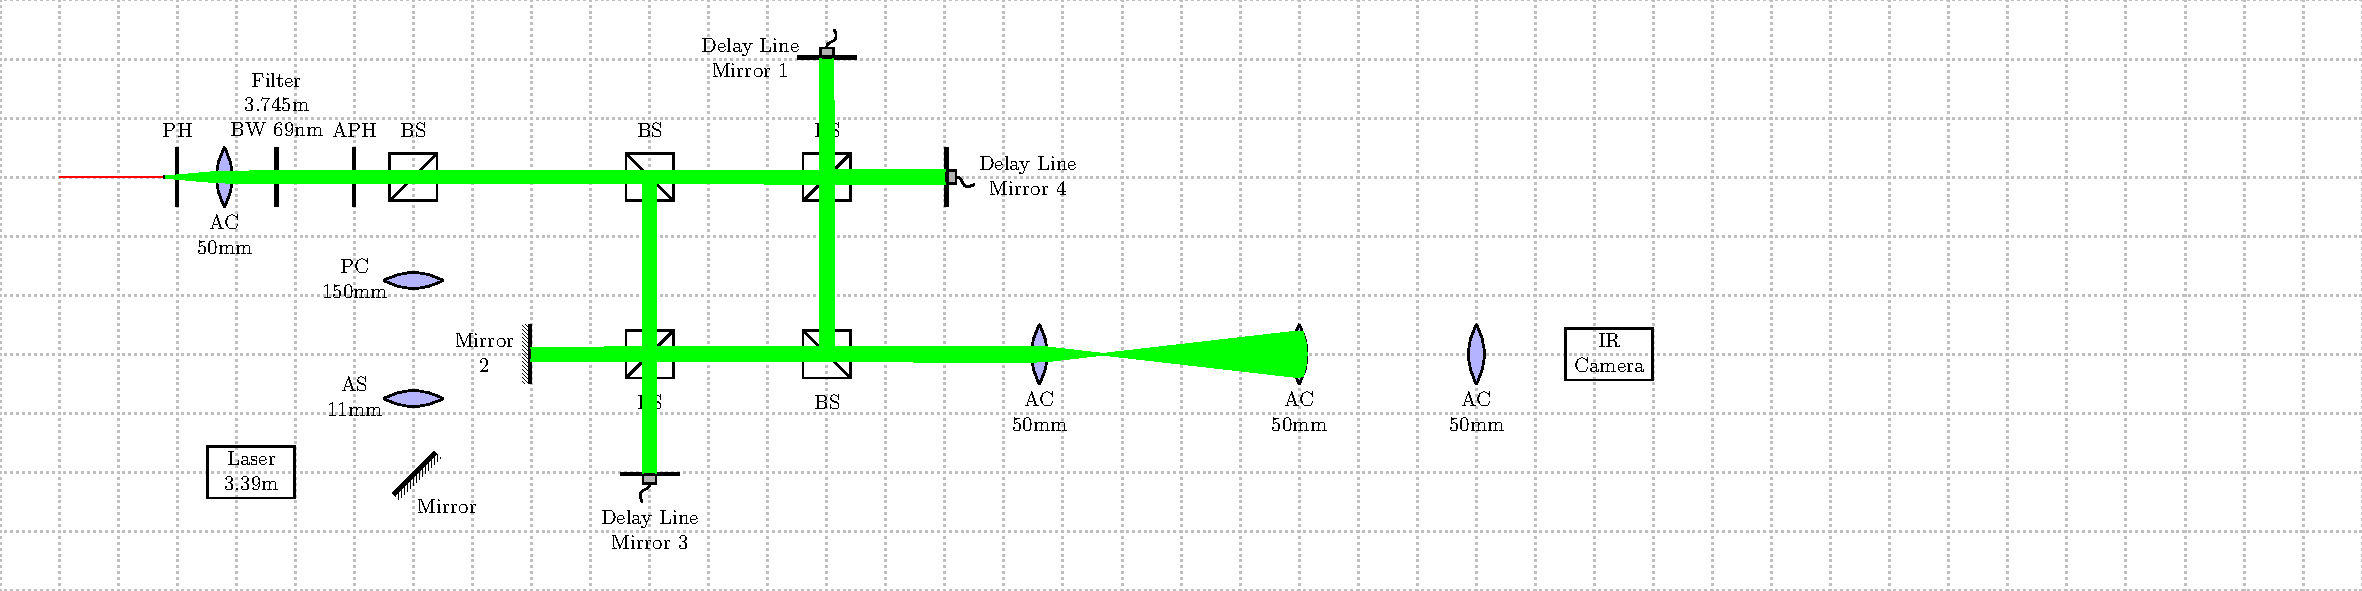
\includegraphics[scale=.53]{../figures/montage.pdf}
 \caption{Experimental setup for characterization of the ZigZag DBC integrated optics chip. The last two lens are used to magnify approximately 8 times. AC = Achromatic, AS = Asphere, PH = PinHole, APH = Adjustable PinHole, BS = Beam-Splitter, PC = Plano-Convex.}
 \label{fig:expersetup}
\end{figure}
 
It has been demonstrated in the previous section that the ZigZag DBC can give accurate results with a bandwidth up to 70nm. The purpose of this part is to verify that experimentally. 
For that purpose the experimental setup represented in Fig.\ref{fig:expersetup} was used. It is a Michelson interferometer with 4 beams. The beams from Mirror 1, 2, 3 and 4 are coupled in the input waveguides 5, 14, 10 and 19 respectively (see Fig \ref{tikz:ZigZagCrossSection} as seen from the input side). 

The DBC used for the characterization is not the one designed in the previous chapter, but is designed to word at 3.4\si{\micro\meter} too. As it appear that at 3.4\si{\micro\meter} all outputs were not illuminated, the source signal was chosen to be a "flat" spectrum signal of 69nm bandwidth centred at 3.745\si{\micro\meter}. If the component was well inscribed in the glass all photometric signal should be symmetrical (i.e the ones from inputs 2,3 and 4,1 should look alike). As can be seen in Fig.\ref{fig:photometries} this is not the case especially for inputs 4, 1. The reason of this is to be found in the writing technique. As the laser inscription technique is not the purpose of this report we will simply explain how it induce birefringence. To inscribe the waveguides the laser write multiple lines that overlap each-other. This overlapping lines make the result dependant of the order of inscription of the waveguides which cause the birefringence effect responsible of the not symmetrical pattern. This has to be verified using a polariser.

\begin{figure}
 \centering
 \includegraphics[scale=.45]{photometries.pdf}
 \caption{The photometric signal of the DBC. As can be seen the signal from input 4 ans 1 are not symmetrical certainly due to birefringence.}
 \label{fig:photometries}
\end{figure}

A second point to explain is the presence of the laser. As the Delay-lines were not very accurate in their movement, the laser was here to calibrate the OPD. Using the fringe spacing of the laser's interferogram, one can reconstruct the real OPD introduced by the delay-line. In order to do so in a First experiment the laser was coupled into the DBC together with the supercontinum source (at 3.8 \si{\micro\meter}). As it appeared that the laser signal was not enough distinguishable from the source signal this technique was not used to obtain the results presented in the following paragraph.  Rather than doing that, as the "apparent wavelength" of the high-frequency component of the interferogram has been demonstrated to be quite the same for all output at 70nm bandwidth, one interferogram was used to calibrate the OPD stating that the fringe spacing was 3.745\si{\micro\meter}. 

This method is valid in the limit of "apparent frequency" not too different from one output to the other. In fact this was verified as for BL-1/2 the apparent wavelength was $3.73\pm0.05\si{\micro\meter}$, $3.73\pm0.04\si{\micro\meter}$ for BL-1/3, $3.70\pm0.08\si{\micro\meter}$ for BL-1/4, $3.78\pm0.04\si{\micro\meter}$ for BL-2/3, $3.75\pm0.05\si{\micro\meter}$ for BL-2/4 and $3.69\pm0.07\si{\micro\meter}$ for BL-3/4. This is of the same order of magnitude than what was seen in simulation. 

In order to characterize the V2PM, the following measurements are performed for each of the 6 baselines (recording frequency = 100Hz, delay line velocity = 0.08 mm/s):
\begin{enumerate}
 \item Record the signal from the moving delay-line alone $I_{DL}$ with the delay-line moving (5000 frames).
 \item Record the photometry from the non-moving input alone $I_{Fix}$.
 \item Record the interferogram (with the 2 beams) $I$
\end{enumerate}

The obtained result is in the form of a cube of frames. In these frames 1 pixel is chosen to be approximately centred on each output in order to be influenced as little as possible by the surroundings waveguides (as explained in the first chapter. This pixel with the magnification system of 8 should be an area of less than $4\times 4 \si{\micro\meter}$ which was too large in simulation but the best doable with the setup. - In the case of the component with fanout, one would have to integrate all the flux by taking an area around the output in order to have high SNR - . Then the data is processed to build the V2PM as follows :
\begin{enumerate}
 \item The noise is filtered in Fourier's space.
 \item The OPD is calculated using a chosen interferogram stating that the fringe spacing should be 3.745µm.
 \item $I_{DL}$ and $I_{Fix}$ are subtracted from the interferogram.
 \item The protocorrection is applied (Eq \ref{eq:photocorpoly})
 \item The envelop of the signal is fitted and the instrumental visibility deduced by it's amplitude
 \item A cosine is fitted to 3 fringes of the interferogram centred at the position of it's maximum to deduce the phase (being $2\pi x/\lambda_0$, $\lambda_0 = 3.745\si{\micro\meter}$ in our case)
 \item the transmission coefficients of the input ($\kappa_{io}$ for input i to output o) are calculated from the photometric data (averaged along the number of frames) by $\kappa_{io} = \frac{I_D(o)}{\sum_{all\_pixels}{I_D(pixel)}}$
 \item The whole V2PM is calculated as in the case of monochromatic light
\end{enumerate}

The condition number of the V2PM resulting with the tested component (numbered 39.7) is 26. The instrumental visibilities for the majority range between 0.6 and 1. In the simulations visibilities were almost all between 90\% and 100\%. The difference is induced by polarisation effects and mostly the birefringence. An histogram of the visibilities is shown in Fig.\ref{fig:hist}. 

\begin{figure}[htbp!]
 \centering
 \includegraphics[scale=.5]{../picture/hist.pdf}
 \caption{Histogram of the experimental instrumental visibilities of the ZigZag DBC number 39.7}
 \label{fig:hist}
\end{figure}


From that V2PM the visibilities and phases of each baselines are retrieved first using directly the data used to calibrate the V2PM, then using data recorded after with 2 or 4 beams in input. The results are presented in the next section. 



    \subsection{Retrieving the visibility function}
    
    
\subsubsection{Using two beams at a time}
Having experimentally determined the V2PM and inverted it to obtain the P2VM, the object visibility and phase are retrieved from the experimental  data. First using the same set of data used to calibrate the V2PM and then using new ones to test the reproducibility of the method. 

The results of the retrieved phases from the data used to calibrate the V2PM matrix are shown on Fig.\ref{fig:retrieved_visi_expe}. These results aren't biased by the calibration of the V2PM because the V2PM only take into account of the visibility and phase of the output interferogram at the position of their maximum. What is flagrant from these results and the simulated ones on a similar component (see \ref{an:retriev}) is that experimentally the retrieved visibility tend to oscillate a lot more around the theoretical one (especially for baseline 14. These oscillations are mostly due to the highly overlapping output signal (as explained in the first chapter), the "apparent wavelength" and the delay-line being not very accurate thus changing the coupling a little from one measurement to the other (this will be verified further). The retrieved visibilities are also a lot impacted by the position of the maximum of the interferogram being not at the same OPD thus leading to the oscillations. With all of these imperfections the retrieve visibility are around the zone of interest (around the maximum) accurate at 10\% for the best baselines to 20\% for the worst. The visibilities retrieved on the second dataset recorded right after the calibration of the V2PM are presented on figure \ref{fig:retrieved_visi_expe2} and are far from as good as the first ones. This is mostly because of the delay-line altering the coupling in their movement and is especially visible on the retrieved visibility for baseline 1-2, 1-3 and 1-4 which were recorded in the same order moving the delay-line of input 1.  


\begin{figure}[htbp!]
 \centering
 \includegraphics[scale=.4]{../picture/retrieve_visi_expe.pdf}
 \caption{Experimentally retrieved visibility from the dataset used to calibrate the V2PM. Baselines numbering 1, 2, 3, 4 refers to the input waveguides (respectively  9, 14, 10 and 19).The x-axis is the OPD in $\mu$m and the y-axis the visibility. The blue line is the actual retrieved data and the orange line the theoretical result. The inset is a zoom of the 50$\mu$m opd around the maximum. }
 \label{fig:retrieved_visi_expe}
\end{figure}

\begin{figure}[htbp!]
 \centering
 \includegraphics[scale=.4]{../picture/retrieve_visi_expe2.pdf}
 \caption{Experimentally retrieved visibility from the data recorded after the V2PM calibration. Baselines numbering 1, 2, 3, 4 refers to the input waveguides (respectively  9, 14, 10 and 19).The x-axis is the OPD in $\mu$m and the y-axis the visibility. The blue line is the actual retrieved data and the orange line the theoretical result. The inset is a zoom of the 50$\mu$m opd around the maximum. }
 \label{fig:retrieved_visi_expe2}
\end{figure}

Concerning the retrieved phase, the results are presented in Fig.\ref{fig:retrieved_phase_expe} for the dataset used to calibrate the V2PM and Fig.\ref{retrieved_phase_expe2} for the second dataset zoomed around the maximum of the interferogram (the "0" OPD). Comparison with the simulated one on the optimised component at 3.4$\mu$m and bandwidth 70nm can be done using Appendix \ref{an:retriev}. It appear that the results are better on the second set of data recorded than on the one used to calibrate the V2PM. This suggest that the phase retrieval is less sensitive to the inperfections of the delay-line and that the uncertainties on it's retrieval are more intrinsic to the noise and the "apparent wavelength" explained before. In all case the residues show a standard deviation to 0 ranging from 0.08 to 0.4 rad. This is equivalent to a sensitivity from $\frac{\lambda_0}{9}$ to $\frac{\lambda_0}{46}$ depending on the baseline and the quality of the calibration ($lambda_0$ being the mid-range wavelength thus 3.745$\mu$m). In the simulated case with the optimised component (70nm bandwidth centered on 3.4$\mu$m wavelength) the residue was about 0.086 rad for all baselines suggesting a possible accuracy of $\frac{\lambda_0}{40}$ for all baselines. To compare Diener et al. presented retrieved visibility ranging from $0.96\pm0.04$ to $1.04\pm0.06$ and phases residue ranging from 0.13 to 0.18 rad in \cite{Diener2017} using a similar component with monochromatic light at 3.39$\mu$m.  

\begin{figure}[htbp!]
 \centering
 \includegraphics[scale=.4]{../picture/retrieve_phase_expe1.pdf}
 \caption{Experimentally retrieved phase from the dataset used to calibrate the V2PM. Baselines numbering 1, 2, 3, 4 refers to the input waveguides (respectively  9, 14, 10 and 19). The blue line is the actual retrieved data, the orange line the theoretical result and the green line the residues (difference between the blue and orange one). $\sigma$ is the standard deviation of the residues in rad. The x-axis is the OPD in $\mu$m and the y-axis the phase in rad. }
 \label{fig:retrieved_phase_expe}
\end{figure}

\begin{figure}[htbp!]
 \centering
 \includegraphics[scale=.4]{../picture/retrieve_phase_expe2.pdf}
 \caption{Experimentally retrieved phase from the data recorded after the V2PM calibration. Baselines numbering 1, 2, 3, 4 refers to the input waveguides (respectively  9, 14, 10 and 19). The blue line is the actual retrieved data, the orange line the theoretical result and the green line the residues (difference between the blue and orange one). $\sigma$ is the standard deviation of the residues in rad. The x-axis is the OPD in $\mu$m and the y-axis the phase in rad. }
 \label{fig:retrieved_phase_expe2}
\end{figure}

For now the experimental demonstration of the feasibility and usability of the Zig-Zag DBC has been done using it to combine only 2 beams at a time. The final purpose of this component beeing to combine 4 telescopes one experimental measurement has been done using the 4 beams.

\subsubsection{Combining the 4 beams}
In order to demonstrate the usability of the Zig-Zag DBC to combine 4 telescopes at a time, the 4 beams where coupled into the component and the P2VM applied to the measured data to retrieve the phases and visibilities of the source. Because of the Delay-line being not very reproducible in its movement only the one that moved the less were used for this measurement (corresponding to input 3, WG 10). The results are sown on Fig.\ref{fig:retrieved_visi_4BL2} and Fig.\ref{fig:retrieved_phase_4BL2}. Only the delay-line of input 3 is scanned thus the visibility and phase of BL 1-2, 1-4 and 2-4 are expected to be constant. The visibility and phase of BL 1-3, 2-3 and 3-4 are supposed to look like the ones of Fig.\ref{fig:retrieved_visi_expe}  and Fig.\ref{fig:retrieved_phase_expe2} respectively. Once again the retrieving algorythm seems to be more accurate on retrieving the phases than the visibilities. This can be explained by the fact that to retrieve the visibilities, 4 different component of the vector $\vec{V}$ are used opposed to 2 to retrieve the phase (see Eq.\ref{eq:banana}) making the phase less sensitive to errors.

Concerning the phase of the 3 scanned baselines, the standard deviation of the residue is less than 0.16 rad which is better than in some case using only 2 beams and the same order of magnitude than reported in \cite{Diener2017}. This can be explain by more amplitude in the interferograms  resulting to higher SNR. The phase of the non scanned baselines shows more volatility (for BLs 1-2 and 1-4 especially). 

Concerning the visibilities of the 3 scanned baselines, the shape of the cardinal sine is visible and the maximum around 1 but the error is up to 40\% in that case.

\begin{figure}[htbp!]
 \centering
 \includegraphics[scale=.4]{../picture/retrieve_visi_4BL2.pdf}
 \caption{Experimentally retrieved visibility from the data recorded after the V2PM calibration. Baselines numbering 1, 2, 3, 4 refers to the input waveguides (respectively  9, 14, 10 and 19). The x-axis is the OPD in $\mu$m and the y-axis the phase in rad. }
 \label{fig:retrieved_visi_4BL2}
\end{figure}

\begin{figure}[htbp!]
 \centering
 \includegraphics[scale=.4]{../picture/retrieve_phase_4BL2.pdf}
 \caption{Experimentally retrieved phase from the data recorded after the V2PM calibration. Baselines numbering 1, 2, 3, 4 refers to the input waveguides (respectively  9, 14, 10 and 19). The blue line is the actual retrieved data, the orange line the theoretical result and the green line the residues (difference between the blue and orange one). $\sigma$ is the standard deviation of the residues in rad. The x-axis is the OPD in $\mu$m and the y-axis the phase in rad. }
 \label{fig:retrieved_phase_4BL2}
\end{figure}

The retrieval of the phase and visibility of a source using the ZigZag-DBC have been demonstrated to be as accurate using a broad-band source of 70nm with similar degree of accuracy than using monochromatic light as reported in \cite{Diener2017} using 2 beams at a time. In the case of using 4 beams the method used showed lower accuracy on retrieving the visibilities. We are convinced that the variation of the coupling due to the delay-lines being not very accurate contributed a lot to the errors and we are convinced that better results could be obtained with better delay-lines (as the simulations showed far better accuracy) and with the component with fanout as suggested the simulations.   

    
\section*{Conclusion and Further-work}

\backmatter
\appendix
\section{Appendix}
    \subsection{The condition number}\label{an:cond}
    Considering the following system $A\vec{x}=\vec{b}$ where A is the
matrix describing our system (A is a matrix with real coefficients). An error $\vec{\delta x}$ on $\vec{x}$
will lead to an error $\vec{\delta b}$ on $\vec{b}$. The aim is to
know how much bigger or smaller is $\frac{\left\|\vec{\delta x}
  \right\|}{\left\|\vec{x} \right\|}$ compared to $\frac{\left\|\vec{\delta b}
  \right\|}{\left\|\vec{b} \right\|}$ (i.e how much an error is
magnified by the A matrix).

In the case where A in neither symmetric nor square. Then the matrix
$A^TA$ is a square symmetric matrix and Then can be diagonalized. Lets
call $\lambda_i$ and $\vec{u_i}$ its eigenvalues and eigenvectors. We
can write : $$ A^TA \vec{u_i} = \lambda_i \vec{u_i}$$
Moreover $$\left\| A\vec{x}\right\|^2 = \vec{x}^TA^TA\vec{x} =
\left\| \vec{b}\right\|^2$$
So $\left\| \vec{b} \right\|^2 \leq max(|\lambda_i|) \left\| \vec{x}
\right\|^2$ and $\left\| \vec{\delta b} \right\|^2 \geq
min(|\lambda_i|) \left\| \vec{\delta x}
\right\|^2$ and then :
$$\boxed{
\frac{\left\|\vec{\delta x}
  \right\|}{\left\|\vec{x} \right\|} \leq \frac{\sqrt{max(|\lambda_i|)}}{\sqrt{min(|\lambda_i|)}} \frac{\left\|\vec{\delta b}
  \right\|}{\left\|\vec{b} \right\|}
}$$

The number $\frac{\sqrt{max(|\lambda_i|)}}{\sqrt{min(|\lambda_i|)}}$
where $min(|\lambda_i|)$ is the minimal non zero eigenvalue of $A^TA$,
is called the condition number of the A matrix. It means how much an
error on the right part of the system can be magnified by the A matrix.

\newpage
    \subsection{Simulated retrieved Phase and visibility}\label{an:retriev}
    In order to compare the results of Fig.\ref{fig:retrieved_visi_expe} in a more readable way than with Fig.\ref{fig:retrieved_fan} the reader can see the results on the following plot.
    \begin{figure}[htbp!]
     \centering
     \includegraphics[scale=.4]{../picture/retrieve_visi_simu.pdf}
     \caption{The simulated retrieved visibilities of the optimised component at $\lambda=3.4\si{\micro\meter}$ and bandwidth=70nm. The x-axis is the OPD in µm and the y-axis the visibility. Baseline numbering follows the ones from Fig.\ref{fig:retrieved_visi_expe}.The blue line is the actual retrieved data and the orange line the theoretical result.}
     \label{an:retrieved_visi_simu}
    \end{figure}
    
    \begin{figure}[htbp!]
     \centering
     \includegraphics[scale=.4]{../picture/retrieve_phase_simu.pdf}
     \caption{The simulated retrieved phases of the optimised component at $\lambda=3.4\si{\micro\meter}$ and bandwidth=70nm. The x-axis is the OPD in µm and the y-axis the phase in rad. Baseline numbering follows the ones from Fig.\ref{fig:retrieved_phase_expe}.The blue line is the actual retrieved data the orange line the theoretical result and the green line the residues (difference between the blue and orange one). $\sigma$ is the standard deviation to 0 of the residues in rad.}
     \label{an:retrieved_phase_simu}
    \end{figure}

\newpage
\printglossary

\newpage
\bibliographystyle{alpha}
\bibliography{biblio}

\end{document}    
